\documentclass{standalone}
\usepackage{tikz}
\usetikzlibrary{calc}
\usetikzlibrary{matrix,positioning,arrows.meta}

\begin{document}
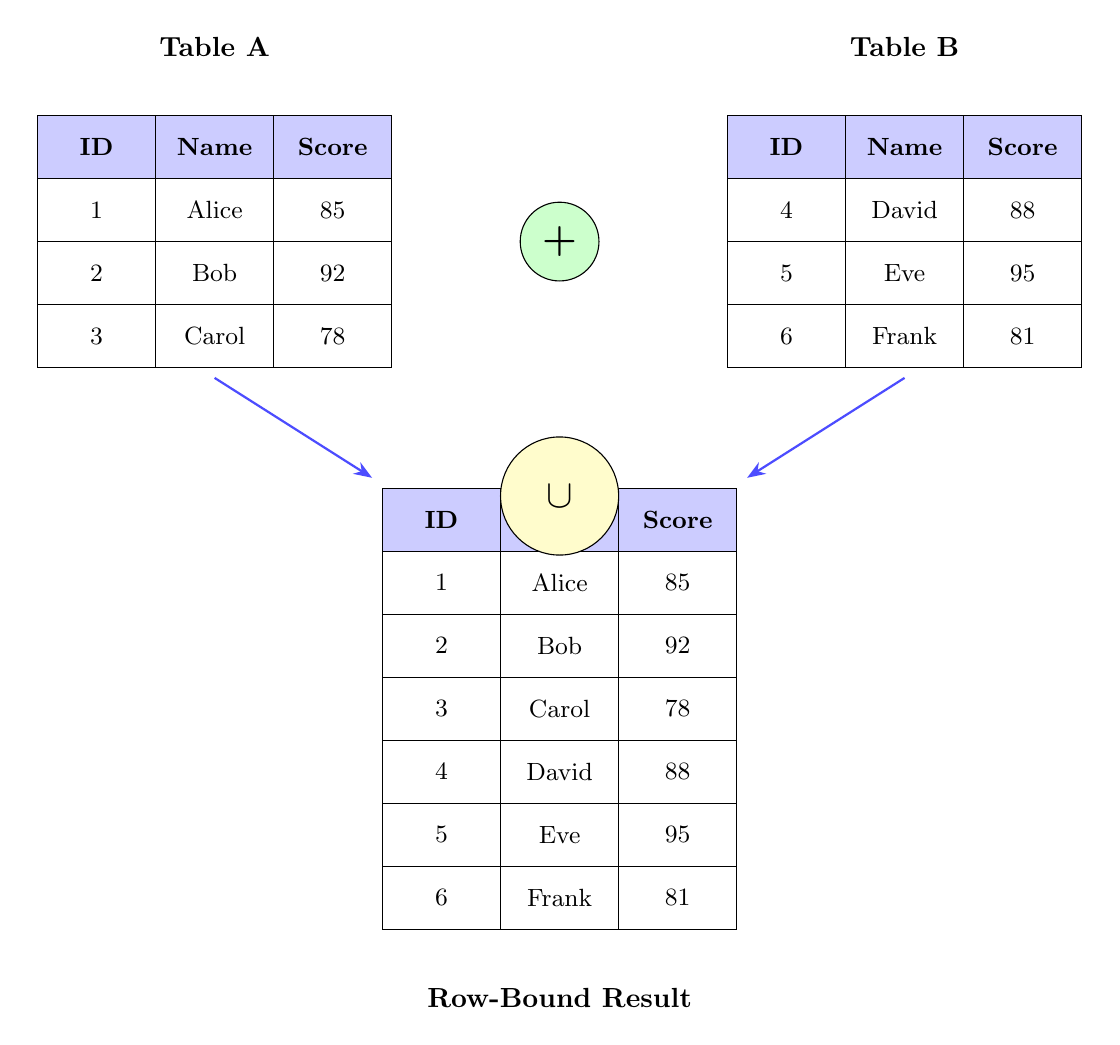
\begin{tikzpicture}[
    table/.style={
        matrix of nodes,
        nodes={
            draw,
            minimum width=1.5cm,
            minimum height=0.8cm,
            anchor=center,
            font=\small
        },
        column sep=-\pgflinewidth,
        row sep=-\pgflinewidth,
    },
    header/.style={fill=blue!20, font=\small\bfseries},
    data/.style={fill=white},
    arrow/.style={-Stealth, thick, blue!70}
]

% Table 1 (top left)
\matrix[table] (table1) {
    |[header]| ID & |[header]| Name & |[header]| Score \\
    |[data]| 1 & |[data]| Alice & |[data]| 85 \\
    |[data]| 2 & |[data]| Bob & |[data]| 92 \\
    |[data]| 3 & |[data]| Carol & |[data]| 78 \\
};

% Table 2 (top right)
\matrix[table, right=4cm of table1] (table2) {
    |[header]| ID & |[header]| Name & |[header]| Score \\
    |[data]| 4 & |[data]| David & |[data]| 88 \\
    |[data]| 5 & |[data]| Eve & |[data]| 95 \\
    |[data]| 6 & |[data]| Frank & |[data]| 81 \\
};

% Merged table (bottom center)
\matrix[table, below=3cm of $(table1)!0.5!(table2)$] (merged) {
    |[header]| ID & |[header]| Name & |[header]| Score \\
    |[data]| 1 & |[data]| Alice & |[data]| 85 \\
    |[data]| 2 & |[data]| Bob & |[data]| 92 \\
    |[data]| 3 & |[data]| Carol & |[data]| 78 \\
    |[data]| 4 & |[data]| David & |[data]| 88 \\
    |[data]| 5 & |[data]| Eve & |[data]| 95 \\
    |[data]| 6 & |[data]| Frank & |[data]| 81 \\
};

% Arrows showing the merge
\draw[arrow] (table1.south) -- (merged.north west);
\draw[arrow] (table2.south) -- (merged.north east);

% Labels
\node[above=0.5cm of table1, font=\bfseries] {Table A};
\node[above=0.5cm of table2, font=\bfseries] {Table B};
\node[below=0.5cm of merged, font=\bfseries] {Row-Bound Result};

% Operation symbol
\node[circle, draw, fill=yellow!20, font=\Large\bfseries, 
      minimum size=1.5cm] at ($(table1.south)!0.5!(table2.south) + (0,-1.5cm)$) {$\cup$};

% Add "+" symbol between tables
\node[circle, draw, fill=green!20, font=\Large\bfseries, 
      minimum size=1cm] at ($(table1.east)!0.5!(table2.west)$) {+};

\end{tikzpicture}
\end{document}